% Prof. Dr. Ausberto S. Castro Vera
% UENF - CCT - LCMAT - Curso de Ci\^{e}ncia da Computa\c{c}\~{a}o
% Campos, RJ,  2022
% Disciplina: Paradigmas de Linguagens de Programa\c{c}\~{a}o
% Aluno: Ricardo Willian Pontes da Silva



\chapter{ Introdu\c{c}\~{a}o}

A linguagem de Programação Python, criada pelo holandês Guido Van Rossum em meados das décadas de 1980 à 1990, se caracteriza por ser do tipo \textit{Very High Level Languagens} (VHLL), ou seja, isso torna a linguagem em alto nível de abstração, porém não voltada apenas para a programação profissional, mas também se destacando em instituições de ensino e por indivíduos autodidatas que desejam ingressar no Python como primeira linguagem. Desta forma, Python também se destaca em detrimento das demais linguagens de programação existentes no mercado pela simplicidade em sua sintaxe, código aberto e também por ser executável em multi-plataformas.
\begin{quote}
Com a evolução da programação, os paradigmas das linguagens também foram se modificando com relação ao tempo, com a linguagem Python não foi diferente, tendo como base o paradigma orientado à objetos, mas também ainda permitindo a criação de códigos na forma procedural, abrangendo diferentes tipos de aplicações (de grandes e pequenas proporções) e desenvolvedores (Profissionais do nível básico ao avançado). Com isso, Python possibilita a migração de um paradigma para outro de forma natural e espontânea por parte do programador.
\end{quote}


   \section{Aspectos hist\'{o}ricos da linguagem Python}
Python surgiu como uma possível solução para as deficiências das linguagens de programação mais aquecidas da época, como C, tendo como filosofia principal a fácil aplicação e intuitiva.   

A seguir, menciona-se alguns aspectos hist\'{o}ricos da linguagem Python, baseados em\cite{Perkovic2016}, \cite{Severance2015},\cite{Labaki}:
\begin{itemize}
  \item Criado por  Guido van Rossum, um holandês de aproximadamente 26 anos em 1982, quando trabalhava no CWI ( Centrum Wiskunde \& Informatica), em Amsterd\~{a}, Holanda.
  \item  Após pensar na linguagem de programação, sua nomeação veio com base no padrão exercido pela organização que seu criador atuava, que se dava por nomenclaturas de animais. Desta forma, Van Rossum, que era fã de um seriado de com\'{e}dia da BBC \textit{Monty Python's Flying Circus} nomeou-a como Python. .
  \item Python 0.9.0 foi lan\c{c}ado em 1991.  Esta vers\~{a}o incluia manipula\c{c}\~{a}o de exce\c{c}\~{o}es, classes, listas e strings. Tamb\'{e}m foram incl\'{\i}dos alguns aspectos de programa\c{c}\~{a}o funcional: lambda, maps flitros e reduce.

  \item  Em 1995, Guido continuou se trabalho sobre Python na Corporation for National Research Initiatives (CNRI) em Reston, Virginia, USA.
  \item Python 1.6 foi lan\c{c}ado no CNRI em
  \item  No ano 2000, Guido e a equipe de desenvolvimento principal do Python foram para BeOpen.com para formar a equipe BeOpen PythonLabs.
  \item Python 2.0 foi lan\c{c}ado no ano 2000
  \item Em 2001, foi formada a PSF (Python Software Foundation), uma organização sem fins lucrativos que mantém e coordena o uso da linguagem. Atualmente, o PSF é suportado por grandes empresas como Google, Microsoft e Globo.com, que também utilizam Python em seus sistemas.
  \item Python 3.o foi lan\c{c}ado em dezembro de 2008 
\end{itemize}

   \begin{figure}[H]
    \begin{center}
        \caption{Logo da Linguagem Python} \label{ling1}
        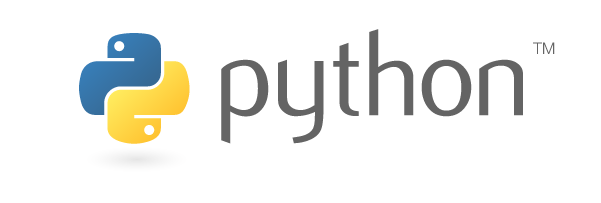
\includegraphics[width=9cm]{python-logo-master-v3-TM.png} \\
        {\tiny \sf Fonte: \cite{VanRossum1995}}
    \end{center}
   \end{figure}

   \section{\'{A}reas de Aplica\c{c}\~{a}o da Linguagem}
   A linguagem Python, diferente da grande maioria em uso atualmente, não possui uma aplicação em específico, podendo ser encontrada no desenvolvimento \textit{Backend/Frontend} como são divididas atualmente áreas mais fomentadas da computação, mas também sendo utilizada em meios como processamento de imagem, aplicações \textit{Mobile, Data Science} e inúmeras outras.\\
   Vale destacar também que, como a linguagem de programação Python é muito versátil, diversas companhias utilizam de sua estrutura para aplicar em seus serviços que serão fornecidos ao cliente. Podemos citar empresas que utilizam-se da linguagem Python: Dropbox, Yahoo, Intel, Cisco, HP , IBM e etc. Como citado por \cite{Silva2019}\\
   A linguagem Python também pode ser integrada com diversas outras linguagens de programação, como Java, JavaScript e C. Desta forma, abrangendo ainda mais o seu uso e o perfil do profissional ao qual irá ser responsável pela aplicação.  

        \subsection{ Big Data}
Com o avanço da tecnologia e a conectividade em praticamente todos os meios populacionais, é necessário um estudo e análise dos dados gerados por essa conexão. A área da tecnologia responsável por essa manipulação é chamada de análise de dados, que se tornará ainda mais necessária para que haja tomadas de decisões assertivas. \\         
Por ser uma linguagem fortemente prototipada, de alto nível, orientada a objetos e dinâmica, o Python é uma das mais famosas linguagens para se trabalhar com manipulação de dados e desenvolvimento científico atuantes no mercado.\cite{McKinney2019}\\ 
Outro fator que contribui para o Python ser largamente utilizado nesse meio de aplicação quantitativa e analítica é a grande quantidade de bibliotecas existentes que auxiliam desde o profissional mais iniciante ao mais experiente, com arquitetura robusta para suportar grandes aplicações.Como algumas dessas bibliotecas, podemos citar, NumPy,Pandas, Matplotlib dentre diversas outras \\

        \subsection{ Orienta\c{c}\~{a}o a objetos}
Python é classificada como uma linguagem orientada a objetos, porém também é permissiva ao desenvolvimento de forma imperativa e funcional, ou seja, dizemos que Python é uma linguagem de multi-paradigmas. O paradigma orientado a objeto é baseado no conceito de classes, objetos,métodos e atributos, que visam representar o mundo real \cite{FBarelli2019}. \\
Nesta linguagem de programação, tudo o que existe é um objeto. Atributos, classes, métodos, números e tudo o que existe em uma linguagem mesmo que não necessariamente orientada a objetos, se torna um objeto ao contrário da programação orientada a procedimentos.\\
Desta forma, a Orientação a Objetos na linguagem Python proporciona uma otimização do tempo, maior qualidade nos projetos e maior clareza de entendimento por parte do programador a qual está desenvolvendo a aplicação. Tais pontos positivos se dão uma vez que a estrutura da Python visa retratar o mais próximo possível de como as coisas se agrupam na vida real.  

        \subsection{Processamento de imagens} 
Pela sua sintaxe de simples entendimento, robustez para grades aplicações e agilidade, o Python é altamente utilizado na área da computação responsável por processar e extrair informações de imagens. Esse processo se faz necessário nos dias atuais uma vez que a automação e inteligência dos aparelhos está cada vez mais presente no cotidiano, como, redares inteligentes, seleção de alimentos, dentre diversas outras.\\
Para realizar essa operações e análises, Python conta com uma grande quantidade de bibliotecas funcionais e uma significativa comunidade para auxiliar o programador. Podemos citar bibliotecas como, NumPy (\textit{Numeric Python}), Scypy (\textit{Cientific Python}), Matplotlib. Ambas têm como função principal operar funções matemáticas de maneira ágil e eficiente, como matrizes e vetores.
Vale destacar também que, tais áreas que envolvem tomadas de decisão como processamento de imagem, inteligência artificial e etc, são tratadas como a nova fase da computação, onde aparelhos serão capazes de se assemelhar com os seres humanos em atividades rotineiras. Desta forma, podemos definir a linguagem Python como sendo uma linguagem do futuro e que possibilitará ao programador se manter atualizado\cite{FBarelli2019}. 